\documentclass{report}

%subject to pathing issues, remember to change
\input{../../pkgs/preamble}
\input{../../pkgs/macros}
\input{../../pkgs/letterfonts}
\usetikzlibrary{trees}

\title{\Huge{CS212}\\ BST tree lab 6 }
\author{\huge{Yan Bogdanovskyy (yawnbo)}}
\date{\today}

\begin{document}

\maketitle
\begin{multicols}{2}
\section*{6.1 Question 1}%
\label{sec: Question 1 }
\textbf{Note that the last half looks terrible but I can't make tikz draw it normally without losing sanity\\}
1. \\ \\
\begin{tikzpicture}[
 every node/.style={circle, draw, minimum size=8mm},
 level distance=15mm,
 level 1/.style={sibling distance=40mm},
 level 2/.style={sibling distance=20mm},
 level 3/.style={sibling distance=10mm},
 level 4/.style={sibling distance=10mm}
]
\node {5}
\end{tikzpicture}
\\
2. \\
\begin{tikzpicture}[
 every node/.style={circle, draw, minimum size=8mm},
 level distance=15mm,
 level 1/.style={sibling distance=40mm},
 level 2/.style={sibling distance=20mm},
 level 3/.style={sibling distance=10mm},
 level 4/.style={sibling distance=10mm}
]
\node {5}
	child {node{2}}
	child[missing]
\end{tikzpicture}
\\
3.\\
\begin{tikzpicture}[
 every node/.style={circle, draw, minimum size=8mm},
 level distance=15mm,
 level 1/.style={sibling distance=40mm},
 level 2/.style={sibling distance=20mm},
 level 3/.style={sibling distance=10mm},
 level 4/.style={sibling distance=10mm}
]
\node {5}
	child{node{2}}
	child{node{8}}
\end{tikzpicture}
\\
4.\\
\begin{tikzpicture}[
 every node/.style={circle, draw, minimum size=8mm},
 level distance=15mm,
 level 1/.style={sibling distance=40mm},
 level 2/.style={sibling distance=20mm},
 level 3/.style={sibling distance=10mm},
 level 4/.style={sibling distance=10mm}
]
\node {5}
	child{node{2}
	child{node{1}} child[missing]}
	child{node{8}}
\end{tikzpicture}
\\
5.\\
\begin{tikzpicture}[
 every node/.style={circle, draw, minimum size=8mm},
 level distance=15mm,
 level 1/.style={sibling distance=40mm},
 level 2/.style={sibling distance=20mm},
 level 3/.style={sibling distance=10mm},
 level 4/.style={sibling distance=10mm}
]
\node {5}
	child{node{2}
		child{node{1}
			child{node{0}}
			child[missing]
		}
		child[missing]
	}
	child{node{8}}
\end{tikzpicture}
\\ \\
6.\\
\begin{tikzpicture}[
 every node/.style={circle, draw, minimum size=8mm},
 level distance=15mm,
 level 1/.style={sibling distance=40mm},
 level 2/.style={sibling distance=20mm},
 level 3/.style={sibling distance=10mm},
 level 4/.style={sibling distance=10mm}
]
\node {5}
	child{node{2}
		child{node{1}
			child{node{0}}
			child[missing]
		}
		child{node{3}}
	}
	child{node{8}}
\end{tikzpicture}
\\
7.\\
\begin{tikzpicture}[
 every node/.style={circle, draw, minimum size=8mm},
 level distance=15mm,
 level 1/.style={sibling distance=40mm},
 level 2/.style={sibling distance=20mm},
 level 3/.style={sibling distance=10mm},
 level 4/.style={sibling distance=10mm}
]
\node {5}
	child{node{2}
		child{node{1}
			child{node{0}}
			child[missing]
		}
		child{node{3}
			child[missing]
			child{node{4}}
		}
	}
	child{node{8}}
\end{tikzpicture}
\\
8.\\
\begin{tikzpicture}[
 every node/.style={circle, draw, minimum size=8mm},
 level distance=15mm,
 level 1/.style={sibling distance=40mm},
 level 2/.style={sibling distance=20mm},
 level 3/.style={sibling distance=10mm},
 level 4/.style={sibling distance=10mm}
]
\node {5}
	child{node{2}
		child{node{1}
			child{node{0}}
			child[missing]
		}
		child{node{3}
			child[missing]
			child{node{4}}
		}
	}
	child{node{8}
		child{node{7}}
		child[missing]
	}
\end{tikzpicture}
\\
9.\\
\begin{tikzpicture}[
 every node/.style={circle, draw, minimum size=8mm},
 level distance=15mm,
 level 1/.style={sibling distance=40mm},
 level 2/.style={sibling distance=20mm},
 level 3/.style={sibling distance=10mm},
 level 4/.style={sibling distance=10mm}
]
\node {5}
	child{node{2}
		child{node{1}
			child{node{0}}
			child[missing]
		}
		child{node{3}
			child[missing]
			child{node{4}}
		}
	}
	child{node{8}
		child{node{7}
			child{node{6}}
			child[missing]
		}
		child[missing]
	}
\end{tikzpicture}
\\
\newpage
10.\\
\begin{tikzpicture}[
 every node/.style={circle, draw, minimum size=8mm},
 level distance=15mm,
 level 1/.style={sibling distance=40mm},
 level 2/.style={sibling distance=20mm},
 level 3/.style={sibling distance=10mm},
 level 4/.style={sibling distance=10mm}
]
\node {5}
	child{node{2}
		child{node{1}
			child{node{0}}
			child[missing]
		}
		child{node{3}
			child[missing]
			child{node{4}}
		}
	}
	child{node{8}
		child{node{7}
			child{node{6}}
			child[missing]
		}
		child{node{9}}
	}
\end{tikzpicture}
\\
11. Final\\
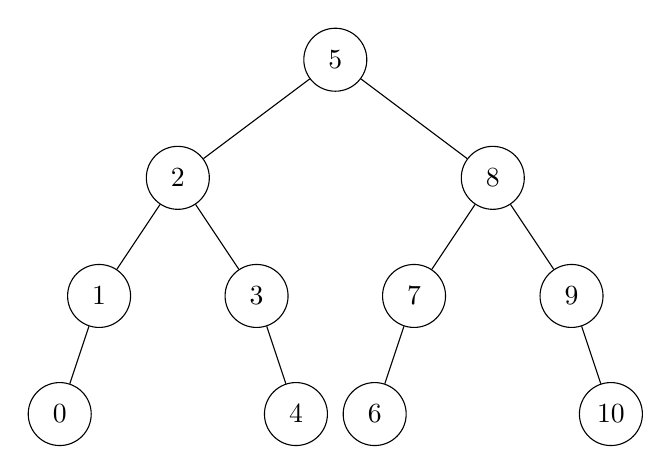
\begin{tikzpicture}[
 every node/.style={circle, draw, minimum size=8mm},
 level distance=15mm,
 level 1/.style={sibling distance=40mm},
 level 2/.style={sibling distance=20mm},
 level 3/.style={sibling distance=10mm},
 level 4/.style={sibling distance=10mm}
]

\node {5}
 child {node {2}
     child {node {1}
         child {node {0}}
         child[missing]
     }
     child {node {3}
         child[missing]
         child {node {4}}
     }
 }
 child {node {8}
     child {node {7}
         child {node {6}}
		 child[missing]
     }
     child {node {9}
         child[missing]
         child {node {10}}
     }
 };
\end{tikzpicture}
\section*{Question 2}%
\label{sec: Question 2 }
1.\\
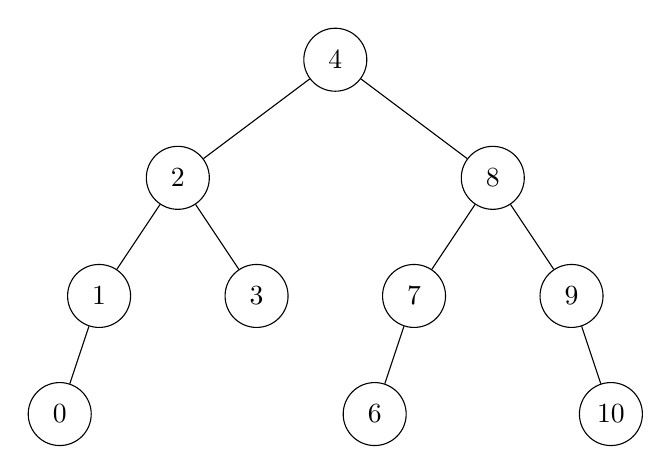
\begin{tikzpicture}[
 every node/.style={circle, draw, minimum size=8mm},
 level distance=15mm,
 level 1/.style={sibling distance=40mm},
 level 2/.style={sibling distance=20mm},
 level 3/.style={sibling distance=10mm},
 level 4/.style={sibling distance=10mm}
]

\node {4}
 child {node {2}
     child {node {1}
         child {node {0}}
         child[missing]
     }
     child {node {3}
     }
 }
 child {node {8}
     child {node {7}
         child {node {6}}
		 child[missing]
     }
     child {node {9}
         child[missing]
         child {node {10}}
     }
 };
\end{tikzpicture}
\\
2.\\
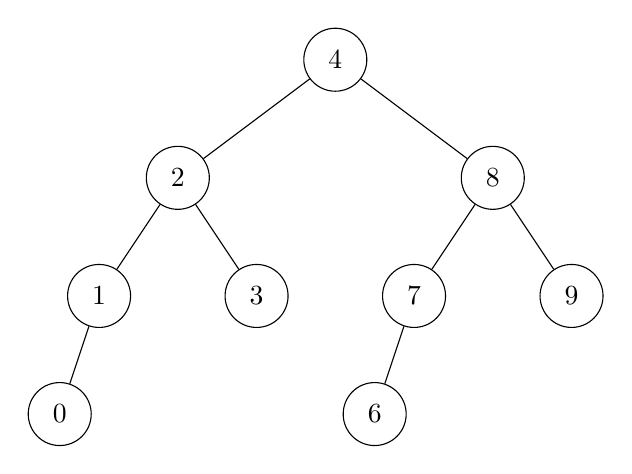
\begin{tikzpicture}[
 every node/.style={circle, draw, minimum size=8mm},
 level distance=15mm,
 level 1/.style={sibling distance=40mm},
 level 2/.style={sibling distance=20mm},
 level 3/.style={sibling distance=10mm},
 level 4/.style={sibling distance=10mm}
]

\node {4}
 child {node {2}
     child {node {1}
         child {node {0}}
         child[missing]
     }
     child {node {3}
     }
 }
 child {node {8}
     child {node {7}
         child {node {6}}
		 child[missing]
     }
     child {node {9}
     }
 };
\end{tikzpicture}
\\
3.\\
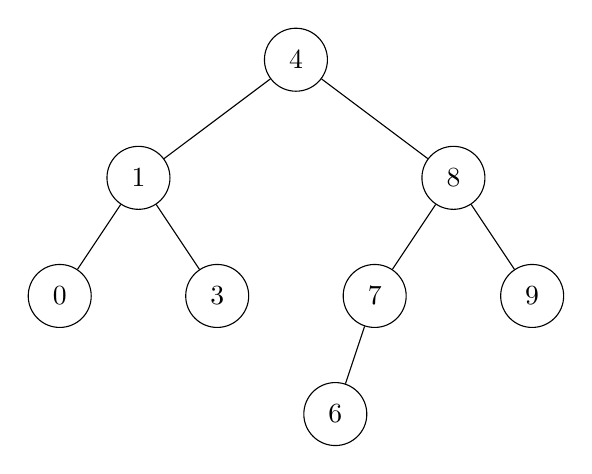
\begin{tikzpicture}[
 every node/.style={circle, draw, minimum size=8mm},
 level distance=15mm,
 level 1/.style={sibling distance=40mm},
 level 2/.style={sibling distance=20mm},
 level 3/.style={sibling distance=10mm},
 level 4/.style={sibling distance=10mm}
]

\node {4}
 child {node {1}
     child {node {0}
     }
     child {node {3}
     }
 }
 child {node {8}
     child {node {7}
         child {node {6}}
		 child[missing]
     }
     child {node {9}
     }
 };
\end{tikzpicture}
\\4.\\

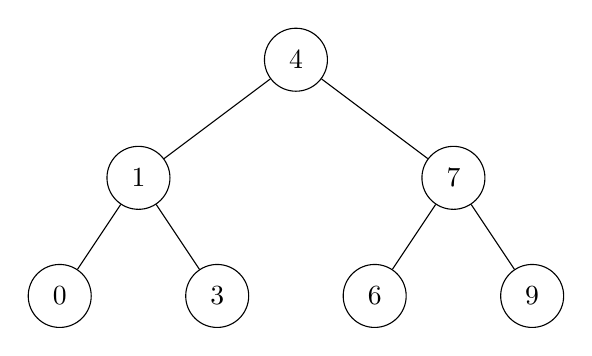
\begin{tikzpicture}[
 every node/.style={circle, draw, minimum size=8mm},
 level distance=15mm,
 level 1/.style={sibling distance=40mm},
 level 2/.style={sibling distance=20mm},
 level 3/.style={sibling distance=10mm},
 level 4/.style={sibling distance=10mm}
]

\node {4}
 child {node {1}
     child {node {0}
     }
     child {node {3}
     }
 }
 child {node {7}
     child {node {6}
     }
     child {node {9}
     }
 };
\end{tikzpicture}
\newpage
\section{Question 3}%
\label{sec: Question 3 }
\\ 1. \\
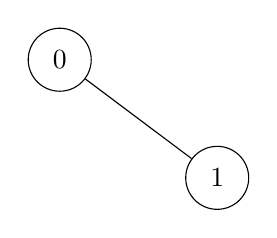
\begin{tikzpicture}[
  every node/.style={circle, draw, minimum size=8mm},
  level distance=15mm,
  level 1/.style={sibling distance=40mm}
]
% Step 2
\node {0}
  child[missing]
  child {node {1}};
\end{tikzpicture}
\\ 2. \\
\begin{tikzpicture}[
  every node/.style={circle, draw, minimum size=8mm},
  level distance=15mm,
  level 1/.style={sibling distance=40mm}
]
% Step 3
\node {0}
  child[missing]
  child {node {1}
    child[missing]
    child {node {2}}
  };
\end{tikzpicture}
\\ 3. \\
\begin{tikzpicture}[
  every node/.style={circle, draw, minimum size=8mm},
  level distance=15mm,
  level 1/.style={sibling distance=40mm},
  level 2/.style={sibling distance=20mm}
]
% Step 4
\node {0}
  child[missing]
  child {node {1}
    child[missing]
    child {node {2}
      child[missing]
      child {node {3}}
    }
  };
\end{tikzpicture}
\\ 4. \\
\begin{tikzpicture}[
  every node/.style={circle, draw, minimum size=8mm},
  level distance=15mm,
  level 1/.style={sibling distance=40mm},
  level 2/.style={sibling distance=20mm},
  level 3/.style={sibling distance=10mm}
]
% Step 5
\node {0}
  child[missing]
  child {node {1}
    child[missing]
    child {node {2}
      child[missing]
      child {node {3}
        child[missing]
        child {node {4}}
      }
    }
  };
\end{tikzpicture}
\\ 5. \\
\begin{tikzpicture}[
  every node/.style={circle, draw, minimum size=8mm},
  level distance=15mm,
  level 1/.style={sibling distance=40mm},
  level 2/.style={sibling distance=20mm},
  level 3/.style={sibling distance=10mm},
  level 4/.style={sibling distance=10mm}
]
% Step 6
\node {0}
  child[missing]
  child {node {1}
    child[missing]
    child {node {2}
      child[missing]
      child {node {3}
        child[missing]
        child {node {4}
          child[missing]
          child {node {5}}
        }
      }
    }
  };
\end{tikzpicture}
\\ 6. \\
\begin{tikzpicture}[
  every node/.style={circle, draw, minimum size=8mm},
  level distance=15mm,
  level 1/.style={sibling distance=40mm},
  level 2/.style={sibling distance=20mm},
  level 3/.style={sibling distance=10mm},
  level 4/.style={sibling distance=10mm}
]
% Step 7
\node {0}
  child[missing]
  child {node {1}
    child[missing]
    child {node {2}
      child[missing]
      child {node {3}
        child[missing]
        child {node {4}
          child[missing]
          child {node {5}
            child[missing]
            child {node {6}}
          }
        }
      }
    }
  };
\end{tikzpicture}
\\ 7. \\
\begin{tikzpicture}[
  every node/.style={circle, draw, minimum size=8mm},
  level distance=15mm,
  level 1/.style={sibling distance=40mm},
  level 2/.style={sibling distance=20mm},
  level 3/.style={sibling distance=10mm},
  level 4/.style={sibling distance=10mm}
]
% Step 8
\node {0}
  child[missing]
  child {node {1}
    child[missing]
    child {node {2}
      child[missing]
      child {node {3}
        child[missing]
        child {node {4}
          child[missing]
          child {node {5}
            child[missing]
            child {node {6}
              child[missing]
              child {node {7}}
            }
          }
        }
      }
    }
  };
\end{tikzpicture}
\\ 8. \\
\begin{tikzpicture}[
  every node/.style={circle, draw, minimum size=8mm},
  level distance=15mm,
  level 1/.style={sibling distance=40mm},
  level 2/.style={sibling distance=20mm},
  level 3/.style={sibling distance=10mm},
  level 4/.style={sibling distance=10mm}
]
% Step 9
\node {0}
  child[missing]
  child {node {1}
    child[missing]
    child {node {2}
      child[missing]
      child {node {3}
        child[missing]
        child {node {4}
          child[missing]
          child {node {5}
            child[missing]
            child {node {6}
              child[missing]
              child {node {7}
                child[missing]
                child {node {8}}
              }
            }
          }
        }
      }
    }
  };
\end{tikzpicture}
\\ 9. \\
\begin{tikzpicture}[
  every node/.style={circle, draw, minimum size=8mm},
  level distance=15mm,
  level 1/.style={sibling distance=40mm},
  level 2/.style={sibling distance=20mm},
  level 3/.style={sibling distance=10mm},
  level 4/.style={sibling distance=10mm}
]
% Step 10
\node {0}
  child[missing]
  child {node {1}
    child[missing]
    child {node {2}
      child[missing]
      child {node {3}
        child[missing]
        child {node {4}
          child[missing]
          child {node {5}
            child[missing]
            child {node {6}
              child[missing]
              child {node {7}
                child[missing]
                child {node {8}
                  child[missing]
                  child {node {9}}
                }
              }
            }
          }
        }
      }
    }
  };
\end{tikzpicture}
\\ 10. \\
\begin{tikzpicture}[
  every node/.style={circle, draw, minimum size=8mm},
  level distance=15mm,
  level 1/.style={sibling distance=40mm},
  level 2/.style={sibling distance=20mm},
  level 3/.style={sibling distance=10mm},
  level 4/.style={sibling distance=10mm}
]
% Step 11
\node {0}
  child[missing]
  child {node {1}
    child[missing]
    child {node {2}
      child[missing]
      child {node {3}
        child[missing]
        child {node {4}
          child[missing]
          child {node {5}
            child[missing]
            child {node {6}
              child[missing]
              child {node {7}
                child[missing]
                child {node {8}
                  child[missing]
                  child {node {9}
                    child[missing]
                    child {node {10}}
                  }
                }
              }
            }
          }
        }
      }
    }
  };
\end{tikzpicture}
\\ 11. \\
\newpage
\section{Question 4}%
\label{sec: Question 4 }
\\ 1.\\
\begin{tikzpicture}[
  every node/.style={circle, draw, minimum size=8mm},
  level distance=15mm,
  level 1/.style={sibling distance=40mm},
  level 2/.style={sibling distance=20mm},
  level 3/.style={sibling distance=10mm},
  level 4/.style={sibling distance=10mm}
]
\node {0}
  child[missing]
  child {node {1}
    child[missing]
    child {node {2}
      child[missing]
      child {node {3}
        child[missing]
        child {node {4}
          child[missing]
          child {node {6}
            child[missing]
            child {node {7}
              child[missing]
              child {node {8}
                child[missing]
                child {node {9}
                  child[missing]
                  child {node {10}}
                }
              }
            }
          }
        }
      }
    }
  };
\end{tikzpicture}
\columnbreak
\\2.\\
% --- Step 2: Remove 10 ---
% 10 is a leaf node; simply remove it.

\begin{tikzpicture}[
  every node/.style={circle, draw, minimum size=8mm},
  level distance=15mm,
  level 1/.style={sibling distance=40mm},
  level 2/.style={sibling distance=20mm},
  level 3/.style={sibling distance=10mm},
  level 4/.style={sibling distance=10mm}
]
\node {0}
  child[missing]
  child {node {1}
    child[missing]
    child {node {2}
      child[missing]
      child {node {3}
        child[missing]
        child {node {4}
          child[missing]
          child {node {6}
            child[missing]
            child {node {7}
              child[missing]
              child {node {8}
                child[missing]
                child {node {9}}
              }
            }
          }
        }
      }
    }
  };
\end{tikzpicture}
\newpage
\\ 3.\\
% --- Step 3: Remove 2 ---
% 2 has only a right child (3), so 3 replaces it.

\begin{tikzpicture}[
  every node/.style={circle, draw, minimum size=8mm},
  level distance=15mm,
  level 1/.style={sibling distance=40mm},
  level 2/.style={sibling distance=20mm},
  level 3/.style={sibling distance=10mm},
  level 4/.style={sibling distance=10mm}
]
\node {0}
  child[missing]
  child {node {1}
    child[missing]
    child {node {3}
      child[missing]
      child {node {4}
        child[missing]
        child {node {6}
          child[missing]
          child {node {7}
            child[missing]
            child {node {8}
              child[missing]
              child {node {9}}
            }
          }
        }
      }
    }
  };
\end{tikzpicture}
\\4.\\
% --- Step 4: Remove 8 ---
% 8 has only a right child (9), so 9 replaces it.

\begin{tikzpicture}[
  every node/.style={circle, draw, minimum size=8mm},
  level distance=15mm,
  level 1/.style={sibling distance=40mm},
  level 2/.style={sibling distance=20mm},
  level 3/.style={sibling distance=10mm},
  level 4/.style={sibling distance=10mm}
]
\node {0}
  child[missing]
  child {node {1}
    child[missing]
    child {node {3}
      child[missing]
      child {node {4}
        child[missing]
        child {node {6}
          child[missing]
          child {node {7}
            child[missing]
            child {node {9}}
          }
        }
      }
    }
  };
\end{tikzpicture}
\end{multicols}
\includegraphics[width=\textwidth]{ss.png}
\end{document}
